\PassOptionsToPackage{dvipsnames,svgnames,x11names}{xcolor}
\documentclass[tikz,border=8pt]{standalone}
\usetikzlibrary{arrows.meta,positioning,calc,shapes,shadows,decorations.pathmorphing,shapes.geometric,backgrounds,decorations.markings,decorations.pathreplacing,decorations.text,fit,shapes.misc,shapes.arrows,matrix,bending,3d,chains,intersections,shapes.symbols,svg.path,shapes.multipart,snakes,shapes.callouts,angles,quotes}
\providecolor{gold}{RGB}{212,175,55}
\providecolor{silver}{RGB}{192,192,192}
\providecolor{bronze}{RGB}{205,127,50}
\providecolor{darkblue}{RGB}{0,0,139}
\providecolor{lightblue}{RGB}{173,216,230}
\providecolor{darkgreen}{RGB}{0,100,0}
\providecolor{lightgreen}{RGB}{144,238,144}
\providecolor{darkred}{RGB}{139,0,0}
\providecolor{navy}{RGB}{0,0,128}
\providecolor{skyblue}{RGB}{135,206,235}
\providecolor{beige}{RGB}{245,245,220}
\providecolor{cream}{RGB}{255,253,208}
\usepackage{amsmath}
\usepackage{amssymb}
\usepackage{fontawesome5}
\usetikzlibrary{fadings,shadows.blur,patterns,patterns.meta}


\usepackage{amsmath}
\usepackage{amssymb}
\usepackage{xcolor}
\usepackage{fontawesome5}

% --- COLOR PALETTE DEFINITION ---
\definecolor{cssengine}{HTML}{6C5CE7}      % Deep Indigo Purple (#6C5CE7)
\definecolor{htmltag}{HTML}{D35400}        % Burnt Orange
\definecolor{shieldred}{HTML}{E74C3C}      % Crimson Forcefield Red (#E74C3C)
\definecolor{successgreen}{HTML}{2ECC71}   % Emerald Green (#2ECC71)
\definecolor{dombg}{HTML}{F8F9FA}          % Ultra-light Slate Gray (#F8F9FA)
\definecolor{domborder}{HTML}{BDC3C7}      % Muted Platinum Gray (#BDC3C7)
\definecolor{svgnode}{HTML}{F39C12}        % Vibrant Amber / Gold (#F39C12)
\definecolor{textdark}{HTML}{2C3E50}       % Midnight Slate Charcoal (#2C3E50)

\begin{document}
\begin{tikzpicture}

% ==============================================================================
% 2. GLOBAL CANVAS & BASELINE BACKGROUND
% ==============================================================================
\fill[white] (-12.9027,-4.9114) rectangle (12.9718,15.0633);

% ==============================================================================
% 3. HEADERS & THE CSSOM ENGINE (Y = 14.0 down to Y = 9.9)
% ==============================================================================
% Main Title
\node[font=\Huge\bfseries\sffamily, text=textdark, align=center] at (-0.0282,13.5633) {Inline SVG vs. External Reference: DOM Integration};

% Sub-title
\node[font=\Large\sffamily, text=textdark!70, align=center] at (-0.0282,12.7633) {Understanding the Topological Barrier to CSS Styling \& The CSSOM};

% CSSOM Box Container
\draw[
    top color=cssengine!20,
    bottom color=cssengine!5,
    draw=cssengine,
    line width=1.5pt,
    rounded corners=8pt,
    drop shadow={opacity=0.3, shadow xshift=0pt, shadow yshift=-3pt}
] (-3.0336,10.1819) rectangle (3.5694,11.4436);

% CSSOM Box Text
\node[font=\Large\bfseries\sffamily, text=cssengine, scale=0.8] at (0, 10.7) {\faIcon{css3-alt}\enspace CSS Object Model (CSSOM)};

% ==============================================================================
% 4 & 5. LEFT PATH: CLOSED RENDERING CONTEXT (EXTERNAL SVG)
% ==============================================================================
% Outer Container Box
\draw[
    top color=dombg!80,
    bottom color=dombg!30,
    draw=domborder,
    line width=1.5pt,
    rounded corners=8pt,
    drop shadow={opacity=0.2, shadow xshift=0pt, shadow yshift=-3pt}
] (-10, 1.2) rectangle (-2, 7.0);

% Top Boundary (Dashed Red Line)
\draw[draw=shieldred, dashed, line width=2pt] (-10, 7.0) -- (-2, 7.0);

% Shield Icon (Mathematically masks dashed line)
\node[font=\Huge, text=shieldred, fill=white, inner sep=2pt] at (-6, 7.0) {\faIcon{shield-alt}};

% Container Title (Safely below shield)
\node[font=\large\bfseries\sffamily, text=textdark!70] at (-6, 6.1) {Closed Rendering Context};

% Inner User-Agent Shadow Root Box
\draw[
    draw=shieldred!60,
    dashed,
    line width=1pt,
    rounded corners=6pt,
    fill=white!40
] (-9.2, 1.5) rectangle (-2.8, 5.5);
\node[font=\scriptsize\ttfamily\bfseries, text=shieldred!80] at (-6.0, 5.1) {[User-Agent Shadow Root]};

% Rasterized Image Box
\draw[
    fill=white,
    draw=textdark!30,
    thick,
    rounded corners=6pt,
    drop shadow={opacity=0.15, shadow xshift=0pt, shadow yshift=-2pt}
] (-8.2, 2.0) rectangle (-3.8, 4.5);
\node[font=\Huge, text=shieldred] at (-6.0, 3.8) {\faImage};
\node[font=\footnotesize\bfseries\sffamily, text=textdark!80, align=center] at (-6.0, 2.8) {Rasterized / Isolated\\[2pt]SVG Payload};

% Code Tag (<img>)
\node[font=\Large\bfseries\ttfamily, text=htmltag] at (-6.0, 8.7) {<img src="graphic.svg">};

% Ingress Path (Segment 1 - Top)
\draw[line width=2pt, cssengine, rounded corners=6pt] (-2,10.0973) -- (-2.0, 9.4) -- (-6.0, 9.4) -- (-6.0, 9.15);

% Ingress Path (Segment 2 - Bottom)
\draw[-Stealth=3mm, line width=2pt, cssengine] (-6.0, 8.25) -- (-6.0, 7.2);

% Payload Pill
\node[
    draw=cssengine!70,
    fill=white,
    rounded corners=3pt,
    inner sep=3pt,
    font=\scriptsize\ttfamily\bfseries,
    text=cssengine,
    drop shadow={opacity=0.15, shadow xshift=0pt, shadow yshift=-1pt}
] at (-4.0, 9.7) {[ fill: \#f39c12 ]};

% Deflection Path & Label
\draw[-Stealth=3mm, shieldred, dashed, line width=1.5pt] (-6.4, 7.3) to[out=150, in=330] (-7.5, 7.8);
\node[font=\small\bfseries\sffamily, text=shieldred, text width=2.8cm, align=center, anchor=east] at (-7.7, 7.8) {Shadow Boundary\\Denies Targeting};

% ==============================================================================
% 4 & 6. RIGHT PATH: UNIFIED DOM TOPOGRAPHY (INLINE SVG)
% ==============================================================================
% Outer Container Box
\draw[
    top color=successgreen!10,
    bottom color=white,
    draw=successgreen,
    line width=1.5pt,
    rounded corners=8pt,
    drop shadow={opacity=0.25, shadow xshift=0pt, shadow yshift=-3pt}
] (2, 1.2) rectangle (10, 7.0);

% Top Boundary (Solid Green Line)
\draw[draw=successgreen, line width=2pt] (2, 7.0) -- (10, 7.0);

% Unlock Icon (Mathematically masks top border)
\node[font=\Large, text=successgreen!80!black, fill=white, inner sep=2pt] at (6, 7.0) {\faUnlock};

% Container Title (Safely below unlock icon)
\node[font=\large\bfseries\sffamily, text=successgreen!80!black] at (6, 6.1) {Unified Document Object Model (DOM)};

% Code Tag (<svg>...)
\node[font=\Large\bfseries\ttfamily, text=htmltag] at (6.0, 8.7) {<svg> ... <path> ... </svg>};

% Ingress Path (Segment 1 - Top)
\draw[line width=2pt, cssengine, rounded corners=6pt] (2,10.0973) -- (2.0, 9.4) -- (6.0, 9.4) -- (6.0, 9.15);

% Ingress Path (Segment 2 - Bottom)
\draw[-Stealth=3mm, line width=2pt, cssengine] (6.0, 8.25) -- (6.0, 7.2);
\draw[-Stealth=3mm, line width=1.5pt, cssengine] (6, 6.7) -- (6, 5.5);

% Payload Pill
\node[
    draw=cssengine!70,
    fill=white,
    rounded corners=3pt,
    inner sep=3pt,
    font=\scriptsize\ttfamily\bfseries,
    text=cssengine,
    drop shadow={opacity=0.15, shadow xshift=0pt, shadow yshift=-1pt}
] at (4.0, 9.7) {[ :hover ]};

% Cascade Allowed Label
\node[font=\small\bfseries\sffamily, text=cssengine, text width=3cm, align=center] at (9.0, 7.8) {Deep Cascade \&\\Inheritance Allowed};

% DOM Nodes (Absolute Grid)
\node[rectangle, fill=svgnode!20, draw=svgnode, thick, rounded corners=4pt, inner sep=5pt, font=\ttfamily\small, drop shadow={opacity=0.15, shadow xshift=0pt, shadow yshift=-1pt}] (in_svg) at (6.0, 5.0) {<svg id="hero">};
\node[rectangle, fill=svgnode!20, draw=svgnode, thick, rounded corners=4pt, inner sep=5pt, font=\ttfamily\small, drop shadow={opacity=0.15, shadow xshift=0pt, shadow yshift=-1pt}, scale=0.8] (in_g1)  at (4.5, 3.4) {<g class="layer">};
\node[rectangle, fill=svgnode!20, draw=svgnode, thick, rounded corners=4pt, inner sep=5pt, font=\ttfamily\small, drop shadow={opacity=0.15, shadow xshift=0pt, shadow yshift=-1pt}, scale=0.8] (in_g2)  at (7.5, 3.4) {<g class="ui">};
\node[rectangle, fill=svgnode!40, draw=svgnode, thick, rounded corners=4pt, inner sep=5pt, font=\ttfamily\small, drop shadow={opacity=0.15, shadow xshift=0pt, shadow yshift=-1pt}, scale=0.8] (in_p1)  at (3.5, 1.8) {<path>};
\node[rectangle, fill=svgnode!40, draw=svgnode, thick, rounded corners=4pt, inner sep=5pt, font=\ttfamily\small, drop shadow={opacity=0.15, shadow xshift=0pt, shadow yshift=-1pt}, scale=0.8] (in_p2)  at (5.5, 1.8) {<polygon>};
\node[rectangle, fill=svgnode!40, draw=svgnode, thick, rounded corners=4pt, inner sep=5pt, font=\ttfamily\small, drop shadow={opacity=0.15, shadow xshift=0pt, shadow yshift=-1pt}, scale=0.8] (in_p3)  at (7.5, 1.8) {<circle>};

% Structural Lines (Anchor-to-Anchor Connections)
\draw[line width=1pt, domborder] (in_svg.south) -- (in_g1.north);
\draw[line width=1pt, domborder] (in_svg.south) -- (in_g2.north);
\draw[line width=1pt, domborder] (in_g1.south) -- (in_p1.north);
\draw[line width=1pt, domborder] (in_g1.south) -- (in_p2.north);
\draw[line width=1pt, domborder] (in_g2.south) -- (in_p3.north);

% Orthogonal Cascade Lines
\draw[dashed, cssengine, -Stealth=3mm, line width=1.5pt] (in_svg.west) -- (2.8, 5.0) |- (in_g1.west);
\draw[dashed, cssengine, -Stealth=3mm, line width=1.5pt] (in_g1.west) -- (2.2, 3.4) |- (in_p1.west);
\draw[dashed, cssengine, -Stealth=3mm, line width=1.5pt] (in_g1.east) -- (6.3904,3.4) |- (in_p2.east);
\draw[dashed, cssengine, -Stealth=3mm, line width=1.5pt] (in_svg.east) -- (8.8, 5.0) |- (in_g2.east);
\draw[dashed, cssengine, -Stealth=3mm, line width=1.5pt] (in_g2.east) -- (9.4, 3.4) |- (in_p3.east);

% ==============================================================================
% 7. EXPLANATION BUBBLES (Y = -0.2, Anchor North)
% ==============================================================================
\node[
    fill=white,
    draw=domborder,
    thick,
    rounded corners=8pt,
    text width=8.5cm,
    align=flush left,
    inner sep=12pt,
    drop shadow={opacity=0.2, shadow xshift=0pt, shadow yshift=-4pt},
    anchor=north
] at (-6, -0.2) {
    {\sffamily\textbf{\Large The Isolation Boundary}}\\[6pt]
    {\sffamily\small When SVG is loaded via an \texttt{<img>} tag or CSS \texttt{background-image}, the browser instantiates it within an isolated rendering sandbox. \\[6pt]
    \textbf{Result:} The master document's CSS Object Model cannot traverse this boundary. Complex interactivity, state changes (\texttt{:hover}), and specific geometric fills are locked inside a monolithic black box.}
};

\node[
    fill=white,
    draw=successgreen,
    thick,
    rounded corners=8pt,
    text width=8.5cm,
    align=flush left,
    inner sep=12pt,
    drop shadow={opacity=0.2, shadow xshift=0pt, shadow yshift=-4pt},
    anchor=north
] at (6, -0.2) {
    {\sffamily\textbf{\Large DOM Injection \& The Topography}}\\[6pt]
    {\sffamily\small By parsing the SVG markup directly "inline" into the HTML document, the parser translates every mathematical node into a first-class DOM element (e.g., \texttt{SVGSVGElement}, \texttt{SVGPathElement}). \\[6pt]
    \textbf{Result:} A unified topological tree is created. The CSS cascade flows naturally into the vector geometry, allowing us to target individual paths, vertices, and groups just like standard \texttt{<div>} elements.}
};

\end{tikzpicture}
\end{document}
